\documentclass[xcolor=pdflatex,dvipsnames,table]{beamer}
\usepackage{epsfig,graphicx}
\usepackage{palatino}
\usepackage{fancybox}
\usepackage{relsize}
\usepackage[procnames]{listings}
\usepackage{hyperref}
\usepackage{qtree} % needed?
\usepackage{booktabs}
\usepackage{dirtree}
\usepackage[normalem]{ulem}


% fatter TT font
\renewcommand*\ttdefault{txtt}
% another TT, suggested by Alex
% \usepackage{inconsolata}
% \usepackage[T1]{fontenc} % needed as well?


\newcommand{\scale}{0.7}

\newcommand{\todo}[1]{{\emph{TODO: #1}}}
\newcommand{\martin}[1]{{\color{blue} Martin: #1}}
\newcommand{\abcdef}[1]{{\color{red} Author2: #1}}

% uncomment following for final submission
%\renewcommand{\todo}[1]{}
%\renewcommand{\martin}[1]{}
%\renewcommand{\author2}[1]{}

\newcommand{\code}[1]{{\texttt{#1}}}

\hypersetup{
  linkcolor  = black,
%  citecolor  = blue,
  urlcolor   = blue,
  colorlinks = true,
}

\beamertemplatenavigationsymbolsempty
\setbeamertemplate{footline}[frame number]





\newif\ifbook
% shared in slides and book

\lstdefinelanguage{chisel}{
%  morekeywords={abstract,case,catch,class,def,%
%    do,else,extends,false,final,finally,%
%    for,if,implicit,import,match,mixin,%
%    new,null,object,override,package,%
%    private,protected,requires,return,sealed,%
%    super,this,throw,trait,true,try,%
%    type,val,var,while,with,yield},
%  otherkeywords={=>,<-,<\%,<:,>:,\#,@},
  sensitive=true,
  morecomment=[l]{//},
  morecomment=[n]{/*}{*/},
  morestring=[b]",
  morestring=[b]',
  morestring=[b]"""
}

\usepackage{color}
\definecolor{dkgreen}{rgb}{0,0.6,0}
\definecolor{gray}{rgb}{0.5,0.5,0.5}
\definecolor{mauve}{rgb}{0.58,0,0.82}

% Default settings for code listings
%\ifbook
\lstset{%frame=lines,
  language=chisel,
  aboveskip=3mm,
  belowskip=3mm,
  showstringspaces=false,
  columns=fixed, % basewidth=\mybasewidth,
  basicstyle={\small\ttfamily},
  numbers=none,
  numberstyle=\footnotesize,
  % identifierstyle=\color{red},
  breaklines=true,
  breakatwhitespace=true,
  procnamekeys={def, val, var, class, trait, object, extends},
  % procnamestyle=\ttfamily,
  tabsize=2,
  float
}
%\else
%\lstset{%frame=lines,
%  language=chisel,
%  aboveskip=3mm,
%  belowskip=3mm,
%  showstringspaces=false,
%  columns=fixed, % basewidth=\mybasewidth,
%  basicstyle={\small\ttfamily},
%  numbers=none,
%  numberstyle=\footnotesize\color{gray},
%  % identifierstyle=\color{red},
%  keywordstyle=\color{blue},
%  commentstyle=\color{dkgreen},
%  stringstyle=\color{mauve},
%  breaklines=true,
%  breakatwhitespace=true,
%  procnamekeys={def, val, var, class, trait, object, extends},
%  procnamestyle=\ttfamily\color{red},
%  tabsize=2,
%  float
%}
%\fi

\lstnewenvironment{chisel}[1][]
{\lstset{language=chisel,#1}}
{}

\newcommand{\shortlist}[1]{{\lstinputlisting[nolol]{#1}}}

\newcommand{\longlist}[3]{{\lstinputlisting[float, caption={#2}, label={#3}, frame=tb, captionpos=b]{#1}}}

\newcommand{\verylonglist}[3]{{\lstinputlisting[caption={#2}, label={#3}, frame=tb, captionpos=b]{#1}}}


\title{Finite State Machine with Datapath}
\author{Martin Schoeberl}
\date{\today}
\institute{Technical University of Denmark\\
Embedded Systems Engineering}

\begin{document}

\begin{frame}
\titlepage
\end{frame}

\begin{frame}[fragile]{Overview}
\begin{itemize}
\item Review \code{Vec}
\item Counter based circuits
\item Finite-state machines (FSMs) 
\item FSM with Datapath
\end{itemize}
\end{frame}



\begin{frame}[fragile]{Last Lab}
\begin{itemize}
\item A table to describe a 7-segment decoder
\item Did you finish the exercises?
\item Did you run it on your Basys3 board?
\end{itemize}
\end{frame}

\begin{frame}[fragile]{Vectors and Bundles}
\begin{itemize}
\item You where skeptic on vectors last week
\item Let us repeat it today
\item A vector (\code{Vec}) is an indexable collection
\item Similar to an array in Java
\item Selecting an element for read is a mulitplexer
\item Selecting an element to write is an input to a multiplexer or a register enable
\item Bundles are constructs to structure data
\item Similar to a class in Java or a record in C/VHDL
\end{itemize}
\end{frame}

\begin{frame}[fragile]{A Vector is a Multiplexer}
\begin{itemize}
\item Follwing code is a 3:1 multiplexer
\end{itemize}
\shortlist{../code/vec_mux.txt}
\begin{figure}
  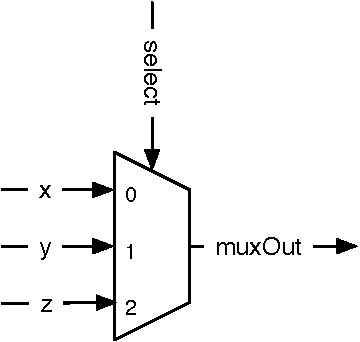
\includegraphics[scale=0.6]{../figures/vec-mux}
\end{figure}
\end{frame}

\begin{frame}[fragile]{A Vector of Registers}
\begin{itemize}
\item Following code shows vectors and registers in action
\end{itemize}
\shortlist{../code/vec_reg.txt}
\begin{itemize}
\item Can you draw the schematic?
\end{itemize}
\end{frame}

\begin{frame}[fragile]{Schematic of the Reg of Vec}
\begin{figure}
  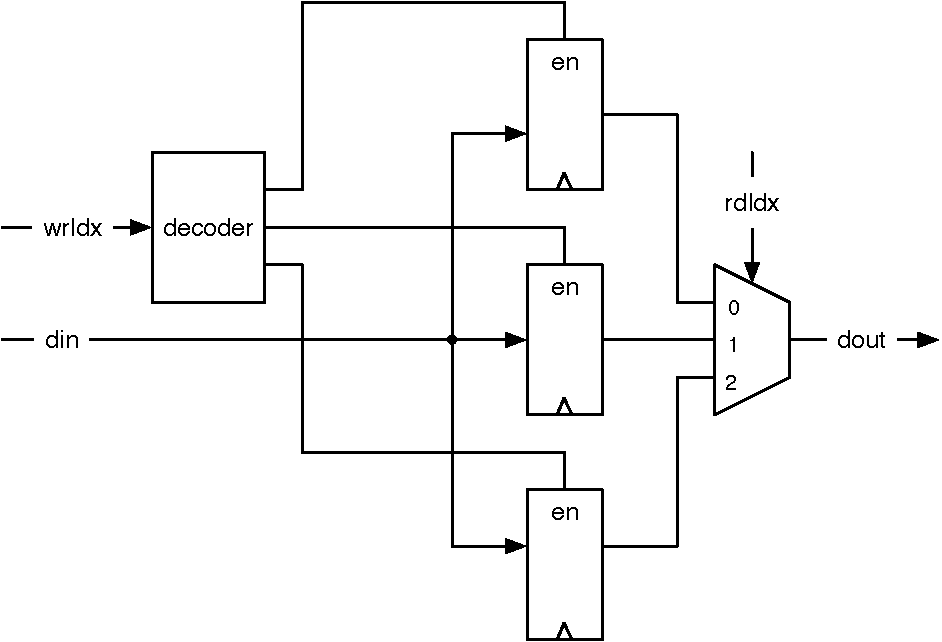
\includegraphics[scale=0.6]{../figures/vec-reg}
\end{figure}
\end{frame}

\begin{frame}[fragile]{Generating Timing with Counters}
\begin{itemize}
\item Generate a \code{tick} at a lower frequency
\item We used it in Lab 1 for the blinking LED
\item We will use it again in next week's lab
\item Use it for driving the display multiplexing at 1~kHz
\end{itemize}
\begin{figure}
  \includegraphics[scale=0.8]{../figures/tick_wave}
\end{figure}
\end{frame}


\begin{frame}[fragile]{The Tick Generation}
\shortlist{../code/sequ_tick_gen.txt}
\end{frame}

\begin{frame}[fragile]{Using the Tick}
\begin{itemize}
\item A counter running at a \emph{slower frequency}
\item By using the \code{tick} as an enable signal
\end{itemize}
\shortlist{../code/sequ_tick_counter.txt}
\end{frame}

\begin{frame}[fragile]{The \emph{Slow} Counter}
\begin{itemize}
\item Incremented every \code{tick}
\end{itemize}
\begin{figure}
  \includegraphics[scale=0.8]{../figures/tick_count_wave}
\end{figure}
\end{frame}

\begin{frame}[fragile]{What is the Use of This \emph{Slow} Counter?}
\begin{itemize}
\item This will be your lab exercise next week
\item Is a preparation for the display multiplexing
\item Then you need to generate a timing of 1 kHz (1 ms)
\end{itemize}
\end{frame}


\begin{frame}[fragile]{Finite-State Machine (FSM)}
\begin{itemize}
\item Has a register that contains the state
\item Has a function to computer the next state
\begin{itemize}
\item Depending on current state and input
\end{itemize}
\item Has an output depending on the state
\begin{itemize}
\item And maybe on the input as well
\end{itemize}
\item Every synchronous circuit can be considered a finite state machine
\item However, sometimes the state space is a little bit too large
\end{itemize}
\end{frame}

\begin{frame}[fragile]{Basic Finite-State Machine}
\begin{itemize}
\item A state register
\item Two combinational blocks
\begin{itemize}
\item Next state logic
\item Output logic
\end{itemize}
\end{itemize}
\begin{figure}
  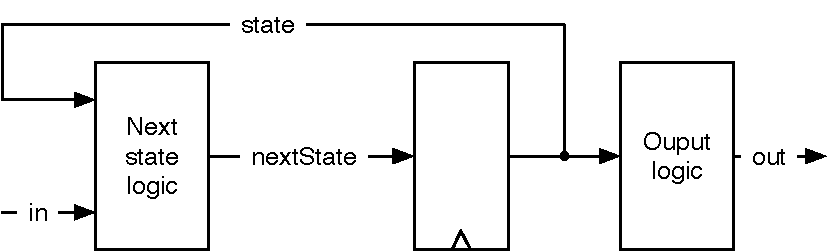
\includegraphics[scale=\scale]{../figures/fsm}
\end{figure}
\end{frame}

\begin{frame}[fragile]{State Diagrams are Convenient}
\begin{figure}
  \includegraphics[scale=\scale]{../figures/state-diag-moore}
\end{figure}
\begin{itemize}
\item States and transitions depending on input values
\item Example is a simple alarm FSM
\item Nice visualization
\item Will not work for large FSMs
\end{itemize}
\end{frame}


\begin{frame}[fragile]{A Mealy FSM}
\begin{itemize}
\item Similar to the former FSM
\item Output also depends in the input
\item Output is \emph{faster}
\item Less composable as we may have combinational circles
\end{itemize}
\begin{figure}
  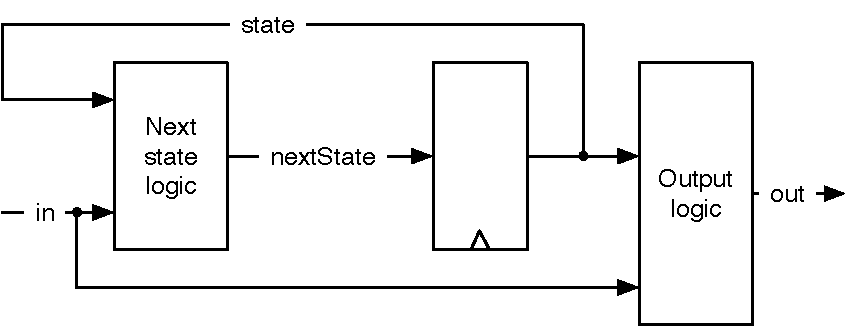
\includegraphics[scale=\scale]{../figures/mealy}
\end{figure}
\end{frame}

\begin{frame}[fragile]{The Mealy FSM for the Rising Edge}
\begin{itemize}
\item Output is also part of the transition arrows
\end{itemize}
\begin{figure}
  \includegraphics[scale=\scale]{../figures/state-diag-mealy}
\end{figure}
\end{frame}

\begin{frame}[fragile]{State Diagram for the Moore Rising Edge Detection}
\begin{itemize}
\item We need three states
\end{itemize}
\begin{figure}
  \includegraphics[scale=\scale]{../figures/state-diag-rising-moore}
\end{figure}
\end{frame}

\begin{frame}[fragile]{Comparing with a Timing Diagram}
\begin{itemize}
\item Moore is delayed by one clock cycle compared to Mealy
\end{itemize}
\begin{figure}
  \includegraphics[scale=1]{../figures/rising}
\end{figure}
\end{frame}

\begin{frame}[fragile]{What is Better?}
\begin{itemize}
\item It depends ;-)
\item Moore is on the save side
\item Moore is composable
\item Mealy has \emph{faster} reaction
\item Both are tools in you toolbox
\item Keep it simple with your vending machine and use a Moore FSM
\end{itemize}
\end{frame}


\begin{frame}[fragile]{FSM with Datapath}
\begin{itemize}
\item A type of computing machine
\item Consists of a finite-state machine (FSM) and a datapath
\item The FSM is the master (the controller) of the datapath
\item The datapath has computing elements
\begin{itemize}
\item E.g., adder, incrementer, constants, multiplexers, ...
\end{itemize}
\item The datapath has storage elements (registers)
\begin{itemize}
\item E.g., sum of money payed, count of something, ...
\end{itemize}
\end{itemize}
\end{frame}

\begin{frame}[fragile]{FSM-Datapath Interaction}
\begin{itemize}
\item The FSM controls the datapath
\begin{itemize}
\item For example, add 2 to the sum
\end{itemize}
\item By controlling multiplexers
\begin{itemize}
\item For example, select how much to add
\item Not adding means selecting 0 to add
\end{itemize}
\item Which value goes where
\item The FSM logic also depends on datapath output
\begin{itemize}
\item Is there enough money payed to release a can of soda?
\end{itemize}
\item FSM and datapath interact
\end{itemize}
\end{frame}


\begin{frame}[fragile]{Popcount Example}
\begin{itemize}
\item An FSMD that computes the popcount
\item Also called the Hamming weight
\item Compute the number of `1's in a word
\item Input is the data word
\item Output is the count
\item Code available at \href{https://github.com/schoeberl/chisel-book/blob/master/src/main/scala/PopCount.scala}{PopCount.scala}
\end{itemize}
\end{frame}

\begin{frame}[fragile]{Popcount Block Diagram}

\begin{figure}
  \includegraphics[scale=\scale]{../figures/popcnt-fsmd}
\end{figure}
\end{frame}


\begin{frame}[fragile]{Popcount Connection}
\begin{columns}
\column{0.6\textwidth}
\begin{itemize}
\item Input \code{din} and output \code{popCount}
\item Both connected to the datapath
\item We need some handshaking
\item For data input and for count output
\end{itemize}
\column{0.4\textwidth}
\begin{figure}
  \includegraphics[scale=0.45]{../figures/popcnt-fsmd}
\end{figure}
\end{columns}
\end{frame}

\begin{frame}[fragile]{Popcount Handshake}
\begin{columns}
\column{0.6\textwidth}
\begin{itemize}
\item We use a ready-valid handshake
\item When data is available valid is asserted
\item When the receiver can accept data ready is asserted
\item Transfer takes place when both are asserted
\item Draw the ready/valid handshake on the black board
\end{itemize}
\column{0.4\textwidth}
\begin{figure}
  \includegraphics[scale=0.45]{../figures/popcnt-fsmd}
\end{figure}
\end{columns}
\end{frame}


\begin{frame}[fragile]{The FSM}
\begin{figure}
  \includegraphics[scale=\scale]{../figures/popcnt-states}
\end{figure}
\begin{itemize}
\item A Very Simple FSM
\item Two transitions depend on input/output handshake
\item One transition on the datapath output
\end{itemize}
\end{frame}

\begin{frame}[fragile]{The Datapath}
\begin{figure}
  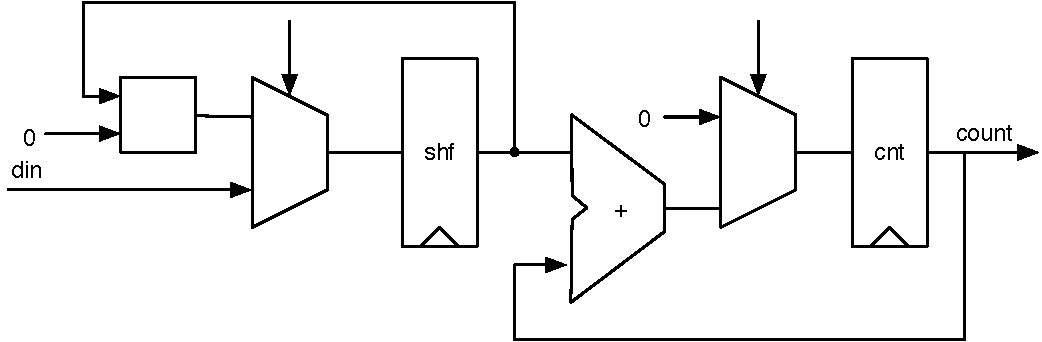
\includegraphics[scale=0.65]{../figures/popcnt-data}
\end{figure}
\end{frame}

\begin{frame}[fragile]{Let's Explore the Code}
\begin{itemize}
\item In \href{https://github.com/schoeberl/chisel-book/blob/master/src/main/scala/PopCount.scala}{PopCount.scala}
\end{itemize}
\end{frame}

\begin{frame}[fragile]{Usage of an FSMD}
\begin{itemize}
\item Maybe the main part your vending machine is an FSMD?
\end{itemize}
\end{frame}


\begin{frame}[fragile]{Functions}
\begin{itemize}
\item Circuits can be encapsulated in functions
\item Each \emph{function call} generates hardware
\item A function is defined with \code{def} \emph{name}
\item Similar to methods in Java
\end{itemize}
\shortlist{../code/components_fn_def.txt}
\shortlist{../code/components_fn_use.txt}
\end{frame}

\begin{frame}[fragile]{More Function Examples}
\begin{itemize}
\item Functions can also contain registers
\item Simple functions can be a single line
\end{itemize}
\shortlist{../code/components_fn_delay.txt}

\begin{chisel}
  def rising(d: Bool) = d && !RegNext(d)
  val edge = rising(cond)
\end{chisel}
\end{frame}

\begin{frame}[fragile]{The Counter as a Function}
\begin{itemize}
\item Longer functions in curly brackets
\item Last value is the return value
\end{itemize}
\shortlist{../code/function_counter.txt}
\end{frame}

\begin{frame}[fragile]{Functional Abstraction}
\begin{itemize}
\item Functions for repeated pieces of logic
\item May contain state
\item Functions may return \emph{hardware}
\item More lightweight than a \code{Module}
\end{itemize}
\end{frame}

%\begin{frame}[fragile]{Functions}
%\begin{itemize}
%\item Example from Patmos execute stage
%\end{itemize}
%\begin{chisel}
%def alu(func: Bits, op1: UInt, op2: UInt): Bits = {
%  val result = UInt(width = DATA_WIDTH)
%  // some more lines...
%  switch(func) {
%    is(FUNC_ADD) { result := sum }
%    is(FUNC_SUB) { result := op1 - op2 }
%    is(FUNC_XOR) { result := (op1 ^ op2).toUInt }
%    // some more lines
%  }
%  result
%}
%\end{chisel}
%\end{frame}

\begin{frame}[fragile]{Parameterization}
\begin{chisel}
class ParamChannel(n: Int) extends Bundle {
  val data = Input(UInt(n.W))
  val ready = Output(Bool())
  val valid = Input(Bool())
}

val ch32 = new ParamChannel(32)
\end{chisel}
\begin{itemize}
\item Bundles and modules can be parametrized
\item Pass a parameter in the constructor
\end{itemize}

\end{frame}
\begin{frame}[fragile]{A Module with a Parameter}
\shortlist{../code/param_adder.txt}
\begin{itemize}
\item Parameter can also be a Chisel type
%\item Can also be a generic type:
%\item \code{class Mod[T <: Bits](param: T) extends...}
\end{itemize}
\end{frame}

\begin{frame}[fragile]{Use the Parameter}
\shortlist{../code/use_param_adder.txt}
\begin{itemize}
\item Can be used for the display multiplexing configuration
\item Different maximum value for the counter for the simulation and for the FPGA
\end{itemize}
\end{frame}


\begin{frame}[fragile]{Today's Lab}
\begin{itemize}
\item Paper \& pencil exercises
\item Exercises on FSMs
\item From the Dally book
\item Just sketch the Chisel code
\item On paper or in a plain text editor
\item As usual, show and discuss your solution with a TA
\end{itemize}
\end{frame}

\begin{frame}[fragile]{Summary}
\begin{itemize}
\item Counters are used to generate timing
\item An FSM can control a datapath, which is an FSMD
\item An FSMD is a computing machine
\item Functions to structure your code
\end{itemize}
\end{frame}


\end{document}

%\begin{frame}[fragile]{xxx}
%\begin{itemize}
%\item yyy
%\end{itemize}
%\end{frame}
